%! Author = joels
%! Date = 27/01/2022

\section{Parser Vertiefung}
\subsection{Syntaxbaum}
\begin{minipage}{0,5\linewidth}
    \textbf{Syntaxbaum:}\\
    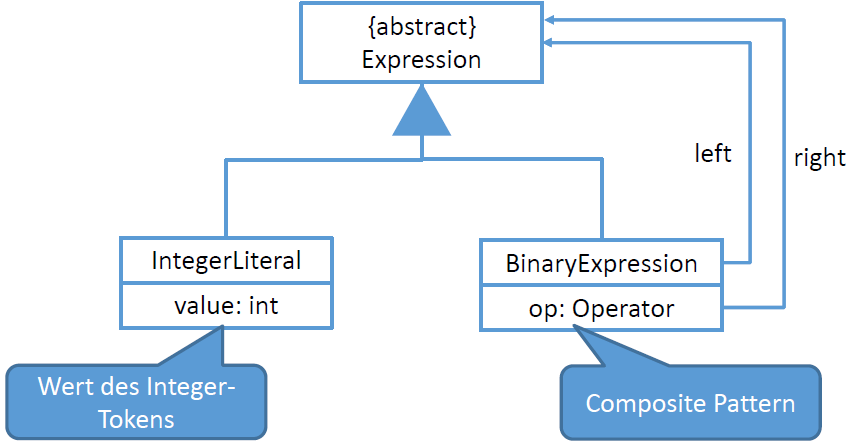
\includegraphics[width=\linewidth]{syntaxbaum}
\end{minipage}
\begin{minipage}{0,5\linewidth}
    \textbf{Syntaxbaum:}\\
    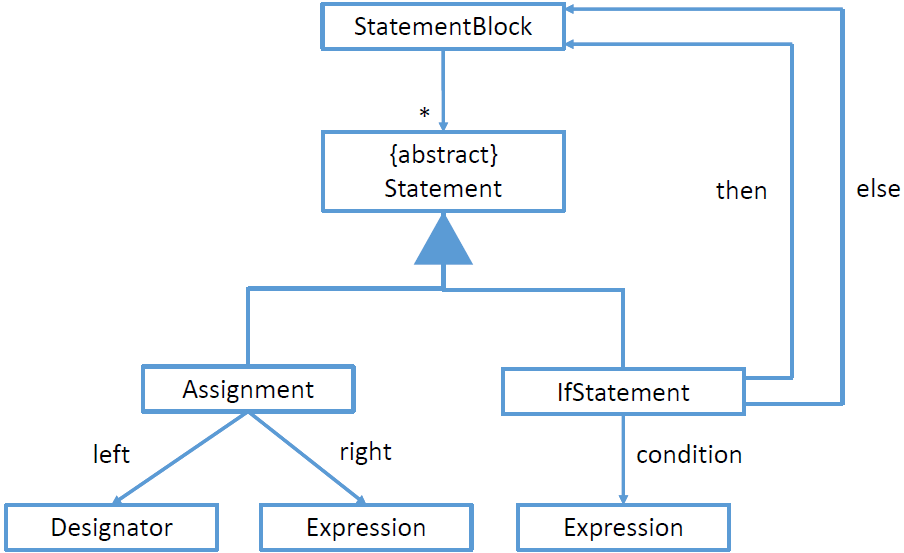
\includegraphics[width=\linewidth]{syntaxbaum_statement}
\end{minipage}

\subsection{Designfragen}
\begin{itemize}[topsep=0pt]
    \itemsep -0.2em
    \item Abstrakt vs. konkret
    \SubItem{Abstract Syntax Tree bei Eigendesign}
    \SubItem{Concrete Syntax Tree bei generiertem Parser}
    \item Weitere Expression-Subklassen
    \SubItem{UnaryExpression (z.B. für -3 oder +4)}
    \SubItem{Andere Literal-Typen (z.B. boolean, string)}
    \SubItem{Designator (z.B. für x oder y[0].z)}
    \item Source Code Positionen merken
    \SubItem{Für fehlermeldungen und Debugging}
    \SubItem{Von Lexer-Symbolstrom übernehmen}
\end{itemize}

\subsubsection{Term parsen}
\begin{lstlisting}
// Term = Number | \dq(\dq Expression \dq)\dq.
Expression parseTerm() {
    if (isInteger()) {
        int value = readInteger();
        next();
        return new IntegerLiteral(value);
    } else if (is(Tag.OPEN_PARENTHESIS)) {
        next();
        var expression = parseExpression();
        if (is(Tag.CLOSE_PARENTHESIS)) {
            next();
        } else {
            error();
        }
        return expression();
    } else {
        error();
    }
}
\end{lstlisting}

\subsection{Syntaxfehler-Behandlung}
\begin{itemize}[topsep=0pt]
    \itemsep -0.2em
    \item Weitermachen bei Fehler $\rightarrow$ Neuen Einstiegspunkt suchen
    \item Hypothesen nötig
    \SubItem{Interpunktionsfehler sind häufig (z.B. fehlendes Semikolon)}
    \SubItem{Vergessener Operator ist selten (z.B. fehlendes Plus)}
    \item Häufige Fehlerarten
    \SubItem{Fehlendes Symbol wie Semikolon oder Klammer $\rightarrow$ ignorieren}
    \SubItem{Falsches Symbol wie falscher Klammertyp $\rightarrow$ ersetzen}
\end{itemize}
\textbf{Nicht erkannte Fehler:} Müssen vom Semantic Checker geprüft werden\\
\begin{itemize}[topsep=0pt]
    \itemsep -0.2em
    \item Inkompatible Typen
    \item Anzahl Argumente ungleich Anzahl Parameter
    \item Nicht deklarierte Variablen/Methoden
    \item Ungültige Operanden
\end{itemize}